\documentclass[../Main_Include.tex]{subfiles}
\begin{document}
\backgroundsetup{contents={}}  % suprime draft de background en compilación standalone
% ============================
% LABORATORIO 2 — Laboratorio2_1015.tex
% ============================
%
% CONTENIDO:
%   Sec. 1 — Convolución circular de secuencias discretas (N = 5)
%
% DEPENDENCIAS (cargadas desde Main_Include.tex):
%   Preambulo.tex       — paquetes, colores, estilos de código
%   PaginaEstilo.tex    — lstset global
%   EstiloSecciones.tex — \titleformat, fancyhdr
%   Entornos.tex        — cuadropregunta
%
% ============================

% --- Título del encabezado para este informe ---
\newcommand{\tituloinforme}{Transformadas de Fourier Discreta y Rápida — Laboratorio 2}

% ══════════════════════════════════════════════════════════════════════
\section{Convolución circular de secuencias discretas}

Basado en el Ejemplo 2.22 de S. Palani, considerar las siguientes secuencias:

\[
    x_1(n) = \{2,\ 1,\ 2,\ 1\}, \quad n = 0,1,2,3
    \qquad
    x_2(n) = \{1,\ 2,\ 3,\ 4,\ 5\}, \quad n = 0,1,2,3,4
\]

Determinar la convolución circular $x_3(m) = x_1(n) \circledcirc_N x_2(n)$ para $N = 5$.

% ──────────────────────────────────────────────────────────────────────
\subsection*{Resolución analítica}

\subsubsection*{Zero-padding de \boldmath$x_1(n)$}

Como $x_1(n)$ tiene 4 muestras y $x_2(n)$ tiene 5, se agrega un cero al final
para igualar $N = 5$, requerido por la convolución circular de $N$ puntos:

\[
    x_1(n) \xrightarrow{\text{zero-pad}} \{2,\ 1,\ 2,\ 1,\ 0\}, \quad n = 0,1,2,3,4
\]

\subsubsection*{Definición formal}

Dadas dos secuencias discretas de longitud $N$, la convolución circular se define como:

\[
    x_3(m) = x_1(n) \circledcirc_N x_2(n)
    = \sum_{n=0}^{N-1} x_1(n)\, x_2\!\left((m-n)_N\right),
    \qquad m = 0, 1, \dots, N-1
\]

donde $(m-n)_N$ es la operación de índice módulo $N$, que mantiene los índices
dentro del rango $[0,\, N-1]$.

\subsubsection*{Método gráfico — Círculos concéntricos (Palani Fig. 2.11)}

\paragraph{Reglas del método.}
\begin{itemize}[leftmargin=1.5cm, itemsep=2pt]
    \item \textbf{Círculo exterior} (fijo): $x_1(n)$ distribuido en sentido
        \textbf{antihorario (CCW)} a intervalos de $\Delta\theta = 360^\circ/N = 72^\circ$,
        comenzando en $0^\circ$.
    \item \textbf{Círculo interior} (móvil): $x_2(n)$ colocado en sentido
        \textbf{horario (CW)}, emulando la inversión temporal $x_2(-n)$
        implícita en la definición.
    \item \textbf{Cálculo de cada muestra:} se multiplican par a par los valores
        alineados radialmente y se suman los productos.
    \item \textbf{Avance temporal:} para pasar de $m$ a $m+1$, el círculo interior
        rota $72^\circ$ en sentido CCW.
\end{itemize}

% ·· m = 0 ··
\paragraph{Paso $m = 0$ — Sin rotación.}

$x_2(0)$ alineado con $x_1(0)$ en $0^\circ$.

\begin{figure}[H]
    \centering
    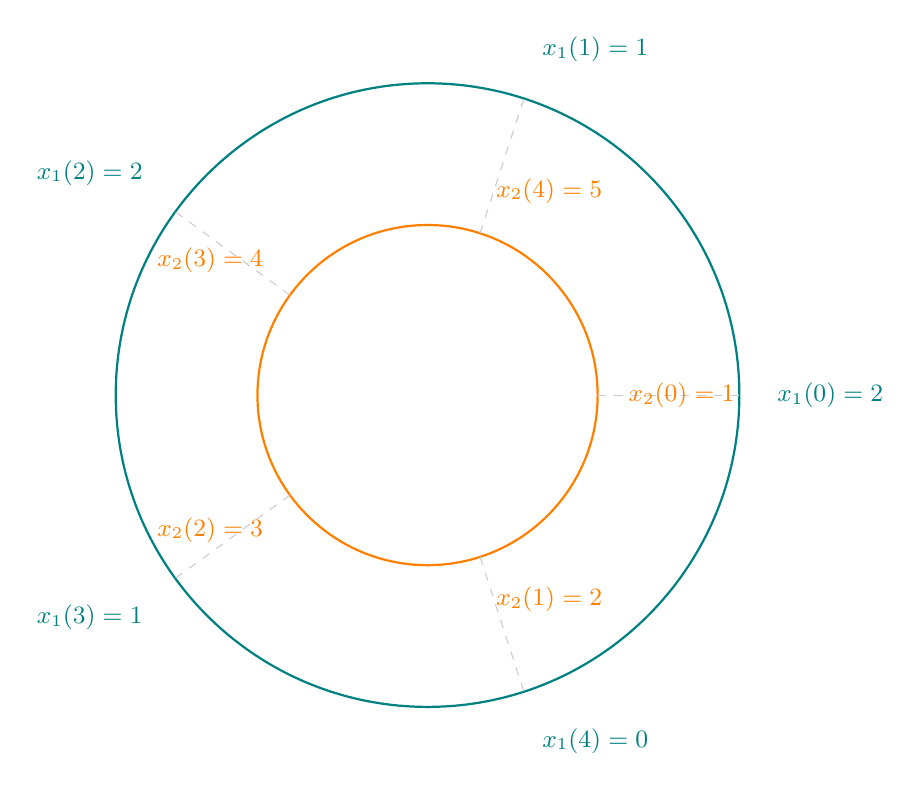
\begin{tikzpicture}[scale=1.8, >=stealth, every node/.style={font=\small}]
        \draw[thick, teal]   (0,0) circle (2.2cm);
        \draw[thick, orange] (0,0) circle (1.2cm);
        \foreach \angle in {0, 72, 144, 216, 288} {
            \draw[dashed, gray!40] (\angle:1.2cm) -- (\angle:2.2cm);
        }
        % Círculo exterior — x1
        \node[teal, anchor=west]       at (0:2.4cm)   {$x_1(0)=2$};
        \node[teal, anchor=south west] at (72:2.4cm)  {$x_1(1)=1$};
        \node[teal, anchor=south east] at (144:2.4cm) {$x_1(2)=2$};
        \node[teal, anchor=north east] at (216:2.4cm) {$x_1(3)=1$};
        \node[teal, anchor=north west] at (288:2.4cm) {$x_1(4)=0$};
        % Círculo interior — x2 (m=0)
        \node[orange, anchor=west]       at (0:1.35cm)   {$x_2(0)=1$};
        \node[orange, anchor=north west] at (288:1.35cm) {$x_2(1)=2$};
        \node[orange, anchor=north east] at (216:1.35cm) {$x_2(2)=3$};
        \node[orange, anchor=south east] at (144:1.35cm) {$x_2(3)=4$};
        \node[orange, anchor=south west] at (72:1.35cm)  {$x_2(4)=5$};
    \end{tikzpicture}
    \caption{Círculos concéntricos para $m = 0$: sin rotación.}
\end{figure}

\[
    x_3(0) = (2{\cdot}1) + (1{\cdot}5) + (2{\cdot}4) + (1{\cdot}3) + (0{\cdot}2)
           = 2 + 5 + 8 + 3 + 0 = \mathbf{18}
\]

% ·· m = 1 ··
\paragraph{Paso $m = 1$ — Rotación de $72°$ CCW.}

$x_2(1)$ queda alineado con $x_1(0)$.

\begin{figure}[H]
    \centering
    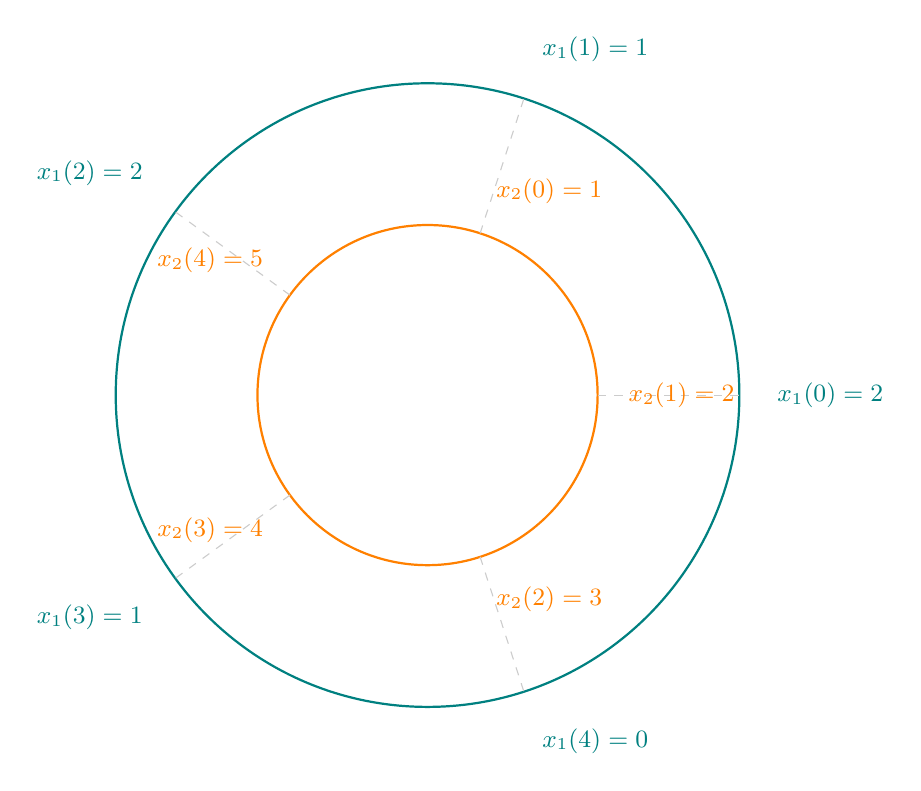
\begin{tikzpicture}[scale=1.8, >=stealth, every node/.style={font=\small}]
        \draw[thick, teal]   (0,0) circle (2.2cm);
        \draw[thick, orange] (0,0) circle (1.2cm);
        \foreach \angle in {0, 72, 144, 216, 288} {
            \draw[dashed, gray!40] (\angle:1.2cm) -- (\angle:2.2cm);
        }
        \node[teal, anchor=west]       at (0:2.4cm)   {$x_1(0)=2$};
        \node[teal, anchor=south west] at (72:2.4cm)  {$x_1(1)=1$};
        \node[teal, anchor=south east] at (144:2.4cm) {$x_1(2)=2$};
        \node[teal, anchor=north east] at (216:2.4cm) {$x_1(3)=1$};
        \node[teal, anchor=north west] at (288:2.4cm) {$x_1(4)=0$};
        \node[orange, anchor=west]       at (0:1.35cm)   {$x_2(1)=2$};
        \node[orange, anchor=north west] at (288:1.35cm) {$x_2(2)=3$};
        \node[orange, anchor=north east] at (216:1.35cm) {$x_2(3)=4$};
        \node[orange, anchor=south east] at (144:1.35cm) {$x_2(4)=5$};
        \node[orange, anchor=south west] at (72:1.35cm)  {$x_2(0)=1$};
    \end{tikzpicture}
    \caption{Círculos concéntricos para $m = 1$: rotación de $72^\circ$ CCW.}
\end{figure}

\[
    x_3(1) = (2{\cdot}2) + (1{\cdot}1) + (2{\cdot}5) + (1{\cdot}4) + (0{\cdot}3)
           = 4 + 1 + 10 + 4 + 0 = \mathbf{19}
\]

% ·· m = 2 ··
\paragraph{Paso $m = 2$ — Rotación acumulada de $144°$ CCW.}

$x_2(2)$ queda alineado con $x_1(0)$.

\begin{figure}[H]
    \centering
    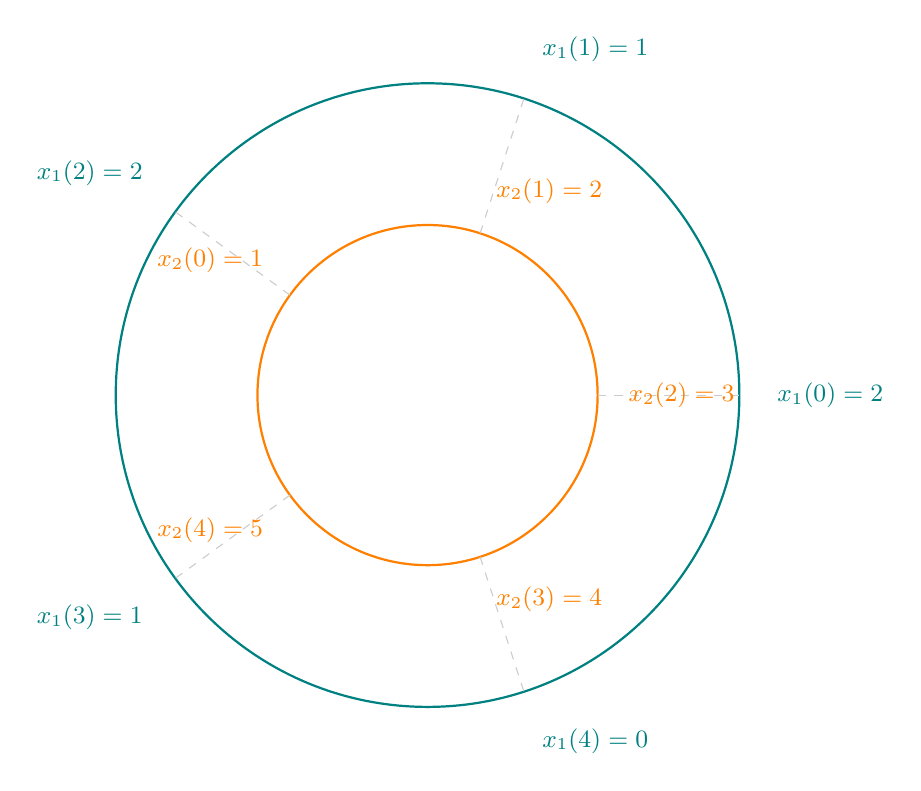
\begin{tikzpicture}[scale=1.8, >=stealth, every node/.style={font=\small}]
        \draw[thick, teal]   (0,0) circle (2.2cm);
        \draw[thick, orange] (0,0) circle (1.2cm);
        \foreach \angle in {0, 72, 144, 216, 288} {
            \draw[dashed, gray!40] (\angle:1.2cm) -- (\angle:2.2cm);
        }
        \node[teal, anchor=west]       at (0:2.4cm)   {$x_1(0)=2$};
        \node[teal, anchor=south west] at (72:2.4cm)  {$x_1(1)=1$};
        \node[teal, anchor=south east] at (144:2.4cm) {$x_1(2)=2$};
        \node[teal, anchor=north east] at (216:2.4cm) {$x_1(3)=1$};
        \node[teal, anchor=north west] at (288:2.4cm) {$x_1(4)=0$};
        \node[orange, anchor=west]       at (0:1.35cm)   {$x_2(2)=3$};
        \node[orange, anchor=north west] at (288:1.35cm) {$x_2(3)=4$};
        \node[orange, anchor=north east] at (216:1.35cm) {$x_2(4)=5$};
        \node[orange, anchor=south east] at (144:1.35cm) {$x_2(0)=1$};
        \node[orange, anchor=south west] at (72:1.35cm)  {$x_2(1)=2$};
    \end{tikzpicture}
    \caption{Círculos concéntricos para $m = 2$: rotación acumulada de $144^\circ$ CCW.}
\end{figure}

\[
    x_3(2) = (2{\cdot}3) + (1{\cdot}2) + (2{\cdot}1) + (1{\cdot}5) + (0{\cdot}4)
           = 6 + 2 + 2 + 5 + 0 = \mathbf{15}
\]

% ·· m = 3 ··
\paragraph{Paso $m = 3$ — Rotación acumulada de $216°$ CCW.}

$x_2(3)$ queda alineado con $x_1(0)$.

\begin{figure}[H]
    \centering
    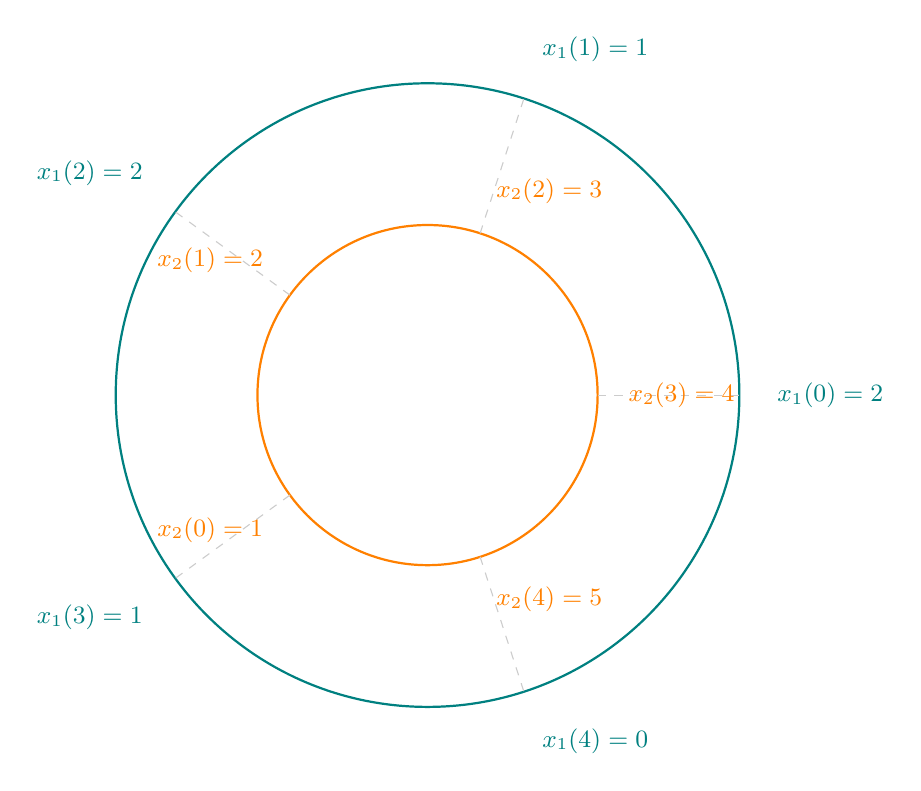
\begin{tikzpicture}[scale=1.8, >=stealth, every node/.style={font=\small}]
        \draw[thick, teal]   (0,0) circle (2.2cm);
        \draw[thick, orange] (0,0) circle (1.2cm);
        \foreach \angle in {0, 72, 144, 216, 288} {
            \draw[dashed, gray!40] (\angle:1.2cm) -- (\angle:2.2cm);
        }
        \node[teal, anchor=west]       at (0:2.4cm)   {$x_1(0)=2$};
        \node[teal, anchor=south west] at (72:2.4cm)  {$x_1(1)=1$};
        \node[teal, anchor=south east] at (144:2.4cm) {$x_1(2)=2$};
        \node[teal, anchor=north east] at (216:2.4cm) {$x_1(3)=1$};
        \node[teal, anchor=north west] at (288:2.4cm) {$x_1(4)=0$};
        \node[orange, anchor=west]       at (0:1.35cm)   {$x_2(3)=4$};
        \node[orange, anchor=north west] at (288:1.35cm) {$x_2(4)=5$};
        \node[orange, anchor=north east] at (216:1.35cm) {$x_2(0)=1$};
        \node[orange, anchor=south east] at (144:1.35cm) {$x_2(1)=2$};
        \node[orange, anchor=south west] at (72:1.35cm)  {$x_2(2)=3$};
    \end{tikzpicture}
    \caption{Círculos concéntricos para $m = 3$: rotación acumulada de $216^\circ$ CCW.}
\end{figure}

\[
    x_3(3) = (2{\cdot}4) + (1{\cdot}3) + (2{\cdot}2) + (1{\cdot}1) + (0{\cdot}5)
           = 8 + 3 + 4 + 1 + 0 = \mathbf{16}
\]

% ·· m = 4 ··
\paragraph{Paso $m = 4$ — Rotación acumulada de $288°$ CCW.}

$x_2(4)$ queda alineado con $x_1(0)$.

\begin{figure}[H]
    \centering
    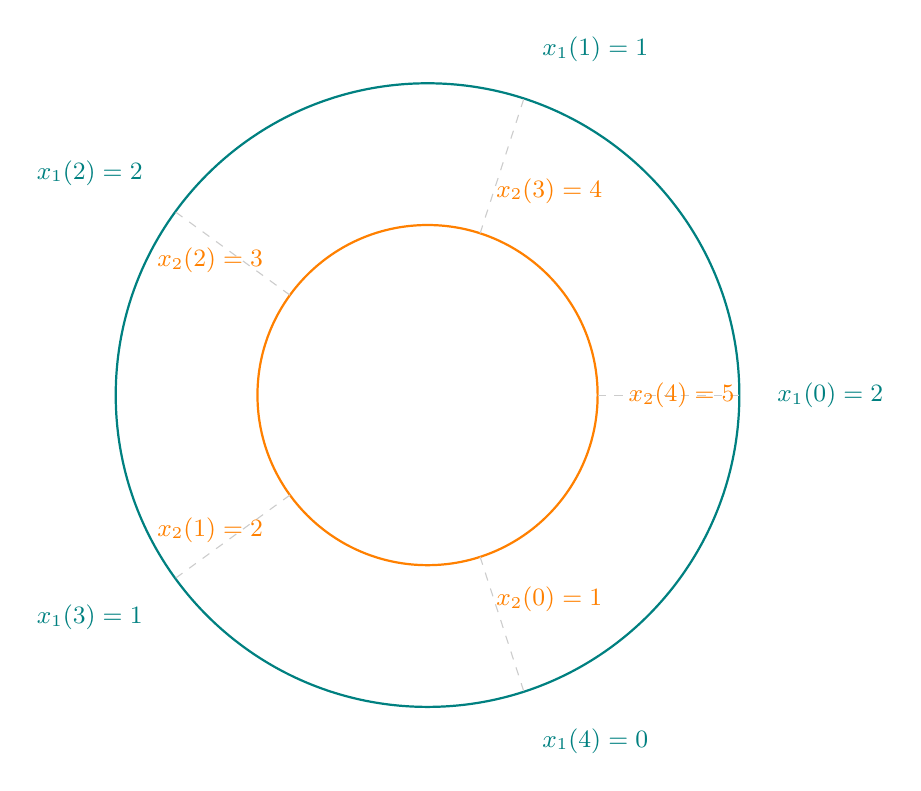
\begin{tikzpicture}[scale=1.8, >=stealth, every node/.style={font=\small}]
        \draw[thick, teal]   (0,0) circle (2.2cm);
        \draw[thick, orange] (0,0) circle (1.2cm);
        \foreach \angle in {0, 72, 144, 216, 288} {
            \draw[dashed, gray!40] (\angle:1.2cm) -- (\angle:2.2cm);
        }
        \node[teal, anchor=west]       at (0:2.4cm)   {$x_1(0)=2$};
        \node[teal, anchor=south west] at (72:2.4cm)  {$x_1(1)=1$};
        \node[teal, anchor=south east] at (144:2.4cm) {$x_1(2)=2$};
        \node[teal, anchor=north east] at (216:2.4cm) {$x_1(3)=1$};
        \node[teal, anchor=north west] at (288:2.4cm) {$x_1(4)=0$};
        \node[orange, anchor=west]       at (0:1.35cm)   {$x_2(4)=5$};
        \node[orange, anchor=north west] at (288:1.35cm) {$x_2(0)=1$};
        \node[orange, anchor=north east] at (216:1.35cm) {$x_2(1)=2$};
        \node[orange, anchor=south east] at (144:1.35cm) {$x_2(2)=3$};
        \node[orange, anchor=south west] at (72:1.35cm)  {$x_2(3)=4$};
    \end{tikzpicture}
    \caption{Círculos concéntricos para $m = 4$: rotación acumulada de $288^\circ$ CCW.}
\end{figure}

\[
    x_3(4) = (2{\cdot}5) + (1{\cdot}4) + (2{\cdot}3) + (1{\cdot}2) + (0{\cdot}1)
           = 10 + 4 + 6 + 2 + 0 = \mathbf{22}
\]

% ──────────────────────────────────────────────────────────────────────
\subsubsection*{Resultado final}

\begin{table}[H]
\centering
\renewcommand{\arraystretch}{1.4}
\begin{tabular}{ccc}
\toprule
\rowcolor{azulprinc}
\textcolor{white}{\textbf{$m$}} &
\textcolor{white}{\textbf{Productos $x_1(n)\,x_2\!\left((m-n)_5\right)$}} &
\textcolor{white}{\textbf{$x_3(m)$}} \\
\midrule
\rowcolor{grisclaro}
$0$ & $2{\cdot}1 + 1{\cdot}5 + 2{\cdot}4 + 1{\cdot}3 + 0{\cdot}2$ & $\mathbf{18}$ \\
$1$ & $2{\cdot}2 + 1{\cdot}1 + 2{\cdot}5 + 1{\cdot}4 + 0{\cdot}3$ & $\mathbf{19}$ \\
\rowcolor{grisclaro}
$2$ & $2{\cdot}3 + 1{\cdot}2 + 2{\cdot}1 + 1{\cdot}5 + 0{\cdot}4$ & $\mathbf{15}$ \\
$3$ & $2{\cdot}4 + 1{\cdot}3 + 2{\cdot}2 + 1{\cdot}1 + 0{\cdot}5$ & $\mathbf{16}$ \\
\rowcolor{grisclaro}
$4$ & $2{\cdot}5 + 1{\cdot}4 + 2{\cdot}3 + 1{\cdot}2 + 0{\cdot}1$ & $\mathbf{22}$ \\
\bottomrule
\end{tabular}
\caption{Desarrollo de la convolución circular término a término.}
\end{table}

\[
    \boxed{x_3(m) = \{18,\ 19,\ 15,\ 16,\ 22\}, \qquad m = 0,1,2,3,4}
\]

\begin{figure}[H]
    \centering
    \rule{\linewidth}{0.4pt}\\[4pt]
    {\small\itshape [Gráfica: $x_3(m)$ — diagrama de tallo, $m = 0,\dots,4$]}\\[4pt]
    \rule{\linewidth}{0.4pt}
    \caption{Resultado de la convolución circular $x_3(m) = x_1(n) \circledcirc_5 x_2(n)$.}
\end{figure}

% ──────────────────────────────────────────────────────────────────────
\subsection*{Código MATLAB}

\lstinputlisting[style=matlab_dark,
    caption={Ejercicio 1 --- Convoluci\'on circular mediante matriz circulante ($N = 5$)},
    label={lst:L2E1}]{Anexos/Lab2/L2E1.m}

\end{document}
